\documentclass[convert={density=140}]{standalone}

\usepackage[T1]{fontenc}
\usepackage[default]{raleway}
\usepackage{hyperref}
%\usefonttheme[onlymath]{serif}% raleway looks ugly in math; this uses standard serif math font

\usepackage{tikz, xcolor}
\usetikzlibrary{shapes.geometric, backgrounds, positioning, decorations.markings} 
\usetikzlibrary{arrows.meta, graphs, shapes.misc} 
\usetikzlibrary{calc}

\definecolor{vq_background}{RGB}{8,31,77}
\definecolor{vq_background2}{RGB}{12,47,116}
\definecolor{vq_background3}{rgb}{0.149,0.388,0.6}
\definecolor{vq_green}{RGB}{0,235,210}
\definecolor{vq_green_light}{RGB}{204,251,246}% green with 80% white added
\definecolor{vq_blue}{RGB}{0,173,234}

\pagecolor{white}

\begin{document}



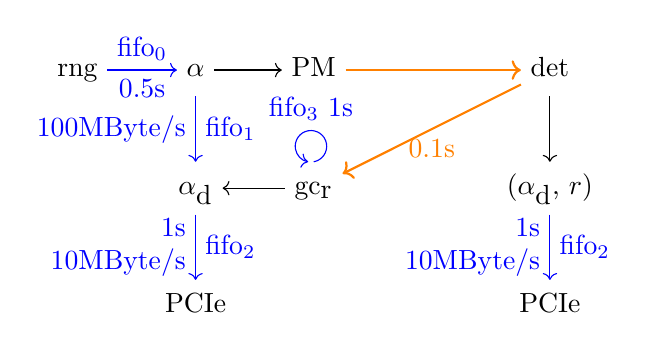
\begin{tikzpicture}[font = \normalsize, node distance=1.5cm, 
    ofast/.style={draw, black, fill=blue!30, minimum size=0.8cm, thin},
    osidechannel/.style={draw, black, fill=blue!30, minimum size=0.8cm, minimum width=1.2cm, thin},
    ofilter/.style={draw, black, fill=red!40, minimum size=0.8cm, thin},
    naked/.style={minimum size = 0},
    fiber/.style={orange, thick},
    fibera/.style={orange, thick, ->},
    fiberbg/.style={white, line width=5pt},
    fifo/.style={blue, ->},
    arrow/.style={->},
    ]

    \coordinate (dx) at (1.5,0);
    \coordinate (c1) at (4,1.5);
    \coordinate (c2) at (6,1.5);
    \coordinate (c3) at (8,1.5);

    \node(rng){\strut rng};
    \node(angle)[right of = rng]{\strut $\alpha$};
    \node(pm)[right of = angle]{\strut PM};
    \node(det)[right of = pm, node distance=3cm]{\strut det};
    \node(gc)[below of = pm]{\strut gc$_\textnormal{r}$};
    \node(dangle)[below of = angle]{\strut $\alpha_\textnormal{d}$};
    \node(dangle2)[below of = det]{\strut ({\strut $\alpha_\textnormal{d}$}, $r$)};
    \node(PCIe)[below of = dangle]{\strut PCIe};
    \node(PCIe2)[below of = dangle2]{\strut PCIe};

    \draw[fifo](rng) -- (angle) node[above, pos=0.5]{fifo$_0$} node[below,pos=0.5]{0.5s};
    \draw[fifo](angle) -- (dangle) node[right, pos=0.5]{fifo$_1$} node[left, pos=0.5, align=right]{100MByte/s};
    \draw[fifo](dangle) -- (PCIe) node[right, pos=0.5]{fifo$_2$} node[left, pos=0.5, align=right]{1s\\10MByte/s};
    \draw[arrow](det) -- (dangle2) ;
    \draw[fifo](dangle2) -- (PCIe2) node[right, pos=0.5]{fifo$_2$} node[left, pos=0.5, align=right]{1s\\10MByte/s};
    
    \draw[fibera](det) -- (gc) node[below, pos=0.5]{0.1s};
    \draw[arrow](angle) -- (pm);
    \draw[arrow](gc) -- (dangle);
    \draw[fibera](pm) -- (det);

    %\draw[arrow,fifo] (gc.north)++(0.05,0) to[out=30, in=0] ++(-0.05,0.3) node[above]{filo$_4$ 1s} to[out=180, in=150] +(-0.05,-0.3);
    \draw[arrow,fifo] (gc.north) arc (-80:260:0.2) node[above, pos=0.5]{fifo$_3$ 1s};

    
    


\end{tikzpicture}



\end{document}











